% !TEX encoding = UTF-8 Unicode
\documentclass[a4paper,12pt]{report}
\newcommand\hmmax{0}
\newcommand\bmmax{0}
		
%Math packages
\usepackage{amsmath, amsfonts, amssymb, amsthm, mathtools}
\usepackage{icomma}
\setcounter{MaxMatrixCols}{20}
%Math packages

%SetFonts
\usepackage{euscript}	 % Шрифт Евклид
\usepackage{mathrsfs} % Красивый матшрифт
\usepackage{dsfont} % Жирный шрифт для множеств чисел
%\usepackage{wasysym} % Для всяких символов
\usepackage{ stmaryrd } %Left \mapsto
\usepackage[T1, T2A]{fontenc}
\usepackage[utf8x]{inputenc}
\usepackage[english, russian]{babel}
%SetFonts

%Graphics
\usepackage{graphicx}
\usepackage{wrapfig}
%Graphics

%Tabular
\usepackage{array, tabularx, tabulary, booktabs}
\usepackage{longtable}
\usepackage{multirow}
%Tabular

%Additional
\newcommand*{\hm}[1]{#1\nobreak\discretionary{}
	{\hbox{$\matsurround=0pt #1$}}{}}
%Additional

%%% Страница
\usepackage{extsizes} % Возможность сделать 14-й шрифт
\usepackage{geometry} % Простой способ задавать поля
\geometry{top=20mm}
\geometry{bottom=20mm}
\geometry{left=15mm}
\geometry{right=15mm}
%
\usepackage{fancyhdr} % Колонтитулы
%\pagestyle{fancy} % Полный набор колонтитулов
\renewcommand{\headrulewidth}{0mm}  % Толщина линейки, отчеркивающей верхний колонтитул
%\lfoot{Нижний левый}
%\rfoot{Нижний правый}
%\rhead{Верхний правый}
%\chead{Верхний в центре}
%\lhead{Верхний левый}
% \cfoot{Нижний в центре} % По умолчанию здесь номер страницы

\usepackage{setspace} % Интерлиньяж
%\onehalfspacing % Интерлиньяж 1.5
%\doublespacing % Интерлиньяж 2
%\singlespacing % Интерлиньяж 1

\usepackage{lastpage} % Узнать, сколько всего страниц в документе.

\usepackage{soul} % Модификаторы начертания

\usepackage{hyperref}
\usepackage[usenames,dvipsnames,svgnames,table,rgb]{xcolor}
\hypersetup{				% Гиперссылки
    unicode=true,           % русские буквы в раздела PDF
    pdftitle={Заголовок},   % Заголовок
    pdfauthor={Автор},      % Автор
    pdfsubject={Тема},      % Тема
    pdfcreator={Создатель}, % Создатель
    pdfproducer={Производитель}, % Производитель
    pdfkeywords={keyword1} {key2} {key3}, % Ключевые слова
    colorlinks=true,       	% false: ссылки в рамках; true: цветные ссылки
    linkcolor=red,          % внутренние ссылки
    citecolor=green,        % на библиографию
    filecolor=magenta,      % на файлы
    urlcolor=cyan           % на URL
}

%\renewcommand{\familydefault}{\sfdefault} % Начертание шрифта



%%%Библиография
\usepackage{cite} % Работа с библиографией
%\usepackage[superscript]{cite} % Ссылки в верхних индексах
%\usepackage[nocompress]{cite} % 
\usepackage{csquotes} % Еще инструменты для ссылок


\usepackage{multicol} % Несколько колонок

\usepackage{tikz} % Работа с графикой
\usepackage{pgfplots}
\usepackage{pgfplotstable}
\usepackage{mathrsfs}
\usetikzlibrary{arrows}

\usepackage{circuitikz}


%reset equation counter after section
\usepackage{chngcntr}

\counterwithin*{equation}{section}
\renewcommand\theequation{\arabic{equation}}
\renewcommand\thesection{\arabic{section}.}
%


%Code listings support
\usepackage{listings}
\lstloadlanguages{[5.2]Mathematica}

\author{Пилипко Михаил Михайлович (а. 448, 2 уч. корп)}
\title{Схемотехника}
\date{2018 год, весенний семестр}
%\date{}							% Activate to display a given date or no date

\begin{document}

\makeatletter
\@addtoreset{chapter}{part}
\makeatother  

\maketitle
\newpage
%\section{}
%\subsection{}
\setcounter{section}{-1}
\section{Литература}
\begin{itemize}
\item Бунтов, Макаров: Микропроцессорные системы. Ч. 1 Цифровые устройства.
\item Угрюмов: Цифровая схемотехника.
\item Морозов, Пилипко: Схемотехника цифровых устройств.
\end{itemize}

\section{Введение}
Будем изучать радиоэлектронные схемы: аналоговые и цифровые.\\
Аналоговый сигнал идёт между $Eп$ и землёй (на самом деле в каких-то внутренних пределах в данном отрезке) по амплитуде, как входной, так и выходной (в одних и тех же пределах).\\
Цель аналоговой схемы: обеспечение рабочей точки внутри заданного диапазона.\\
\\
В цифровой схеме используется 2 уровня сигнала (логические 1 и 0 - земля), переключения между ними как можно более резкие. Между 0 и 1 - зона неопределённости.\\
Требуется обеспечить хорошее различение двух дискретных уровней сигнала.\\
\\
Для преобразования этих схем одну в другую существуют преобразователи: ЦАП и АЦП.\\
АЦП делит временную ось аналогового сигнала на одинаковые отрезки ($Tпреобр$), а ось напряжения делится на некоторые дискретные уровни, кодируемые двоичным кодом (=квантование). На каждом пересечении уровней времени и напряжения аналоговому сигналу сопоставляется как можно более точный цифровой. Чем выше частота дискретизации, тем точнее преобразование. \\
\begin{center}
\begin{tabular}{c | c}
АЦП делает: & ЦАП делает: \\ \hline
1. Дискретизация по времени& \\
2. Квантование по уровню & То же самое, только в обратном порядке\\
3. Кодирование цифровым кодом & \\
\end{tabular}
\end{center}
\section{Системы счисления}
Делятся на позиционные (значение зависит от порядка расположения знаков) или ПСС,  и непозиционные (соответственно, не зависит).\\
\\
Разложение числа по основанию q:\\
$E=e_{n-1}q^{n-1}+...+e_1q^1+e_0q^0$, $n$ - разрядность числа по основанию q.\\
Наиболее популярные основания: 2, 3, 8, 10, 12, 16, 60.\\
Один из критериев сравнения ПСС - удельная информационная плотность (УИП) представления данных.\\
УИП$=q*n$\\
$N=q^n$ - количество представимых чисел.\\
При УИП=30:\\
(график на листочке)\\
По графику видно, что максимальной эффективности можно добиться для систем счисления по основанию $e$. В троичной системе представлять данные удобнее и компактнее, она понятнее, чем двоичная. Естественным образом можно ввести отрицательные числа: 1, 0, -1. Недостатки: нет надёжных и компактных логических, пригодных для троичной логики (с туннельным диодом всё тоже не очень гладко). Оказалось, что проще всего реализовать двоичную логику на транзисторах.\\
\section{Алгебра логики (булева алгебра)}
Переменные имеют только два значения: 0 и 1 (ложь и истина соответственно).\\
Свойства переменных:
\begin{enumerate}
	\item рефлексивность: $x=x$
	\item симметричность: $x=y \to y=x$
	\item транзитивность: $x=y$, $y=z \to x=z$
\end{enumerate}
Функции задаются с помощью таблиц истинности: слева выписываются входные данные и их возможные значения, и им сопоставляются все возможные выходные значения.\\
В рамках булевой логики существует 3 базовые операции:
\begin{enumerate}
\item Конъюнкция (логическое \textbf{И}, логическое умножение). $y=x_1 \cap x_2$\\
\begin{tabular}{ c | c | c }
  $x_1$ & $x_2$ & $y$ \\ \hline
  0 & 0 & 0 \\
  0 & 1 & 0 \\
  1 & 0 & 0 \\
  1 & 1 & 1 \\
\end{tabular}
\item Дизъюнкция (логическое \textbf{ИЛИ}, логическое сложение). $y=x_1 \cup x_2$\\
\begin{tabular}{ c | c | c }
  $x_1$ & $x_2$ & $y$ \\ \hline
  0 & 0 & 0 \\
  0 & 1 & 1 \\
  1 & 0 & 1 \\
  1 & 1 & 1 \\
\end{tabular}
\item Инверсия (логическое \textbf{НЕ}, логическое отрицание). $y=\overline{x}$\\
\begin{tabular}{ c | c }
  $x$ & $y$ \\ \hline
  0 & 1 \\
  1 & 0 \\  
\end{tabular}
\end{enumerate}
Операции 1, 2 возможны для большего числа переменных, причём порядок выполнения операции не повлияет на её итог (свойство ассоциативности для сложения и умножения).\\
$x_1+x_2+...+x_n=y$\\
$x_1*x_2+...*x_n=y$\\
\section{Логические функции и выражения}
Логическая функция - функция логического(-их) аргумента(-ов), которая сама принимает только два значения - 0 или 1. Также называется переключательной.\\
Пусть есть $n$ переменных: $x_1, x_2, ..., x_n$\\
Тогда $N=2^n$ -количество наборов переменных, а количество возможных функций - $2^N$\\
Этот факт можно проиллюстрировать следующей таблицей:\\
\begin{tabular}{ c | c | c | c | c }
  $x$ & $y_1$ & $y_2$ & $y_3$ & $y_4$ \\ \hline
  0 & 0 & 0 & 1 & 1 \\
  1 & 0 & 1 & 0 & 1\\  
\end{tabular}
При этом $y_1=0$, $y_2=x$, $y_3=\overline{x}$, $y_4=1$.\\
Если для некоторых наборов аргументов значение не задано, функция называется недоопределённой.\\
\\
Принцип двойственности логических функций:\\
1. $\overline{x_1+x_2}=y \to \overline{x_1}*\overline{x_2}=y$\\
2. $\overline{x_1*x_2}=y \to \overline{x_1}+\overline{x_2}=y$\\
\\
Это можно доказать, составив соответствующие таблицы истинности. Например, для первого утверждения:\\
\begin{tabular}{ c | c | c | c | c | c | c }
$x_1$ & $x_2$ & $x_1+x_2$ & $\overline{x_1+x_2}$ & $\overline{x_1}$ & $\overline{x_2}$ & $\overline{x_1}*\overline{x_2}$ \\ \hline
0 & 0 & 0 & \textbf{1} & 1 & 1 & \textbf{1} \\
0 & 1 & 1 & \textbf{0} & 1 & 0 & \textbf{0} \\
1 & 0 & 1 & \textbf{0} & 0 & 1 & \textbf{0} \\
1 & 1 & 1 & \textbf{0} & 0 & 0 & \textbf{0} \\
\end{tabular}\\
\\
\\
\textbf{Эквивалентные преобразования логических функций.}\\
Делятся на тождества, законы и операции.
\begin{enumerate}

\item Тождества: 
\subitem{1)}  $x+0=x \quad x*1=x$
\subitem{2)}  $x+1=1 \quad x*0=0$
\subitem{3)} $x+x=x \quad x*x=x$ 
\subitem{4)} $x+\overline{x}=1$ 
\subitem{5)}  $\overline{\overline{x}}=x$

\item Законы: 
\subitem{6)} $x_2+x_1=x_1+x_2 \qquad\qquad\qquad\quad  x_1x_2=x_2x_1$
\subitem{7)} $(x_1+x_2)+x_3=x_1+(x_2+x_3) \quad  (x_1x_2)x_3=x_1(x_2x_3)$
\subitem{8)} $x_1(x_2+x_3)=x_1x_2+x_1x_3 \quad\quad\quad \ x_1+(x_2*x_3)=(x_1+x_2)(x_1+x_3)$ \\
Можно доказать последнее: 
\begin{equation*}
	\begin{aligned}
		&(x_1+x_2)(x_1+x_3)=x_1x_1+x_1x_2+x_1x_3+x_2x_3=x_1(1+x_2+x_3)+x_2x_3=x_1+x_2x_3
	\end{aligned}
\end{equation*}
\item Операции:
\subitem{9)} $\overline{x_1+x_2}=\overline{x_1}*\overline{x_2} \quad \overline{x_1x_2}=\overline{x_1}+\overline{x_2}$  (правила де Моргана)
\subitem{10)} $x_1*x_2+x_1*\overline{x_2}=x_1 \quad (x_1+x_2)(x_1+\overline{x_2})=x_1$ (склеивание)\\

\underline{Однако!}
\begin{equation*}
	\begin{aligned}
		& x_1*\overline{x_2x_3}+x_1*x_2x_3=x_1\\
		& x_1*\overline{x_2}\,\overline{x_3}+x_1*x_2x_3 \not = x_1 \\
	\end{aligned}
\end{equation*}
\subitem{11)} $x_1+x_1x_2=x_1 \quad x_1(x_1+x_2)=x_1$  (поглощение)
\subitem{12)} $x_1*\overline{x_2}+x_2=x_1+x_2 \quad (x_1+\overline{x_2})x_2=x_1x_2$
\end{enumerate}			
\newpage

	
\section{Комбинационная логическая схема}
Входные сигналы ($x_1, x_2, ..., x_n$) будем изображать слева, выход функции  - справа от элемента, реализующего логическую функцию. Также элементу требуется питание и земля, обычно не изображаемые на логических диаграммах, но обязательные на реальных схемах для сборки (на картинке).\\
\begin{center}
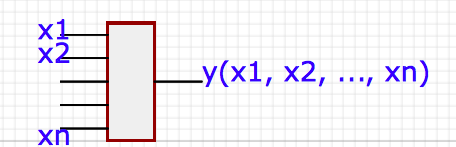
\includegraphics[width=10cm]{logical_element.png}
\end{center}
Пример: мажоритарная функция - каких значений на входных данных будет больше, таким будет выходное значение (на картинке).\\
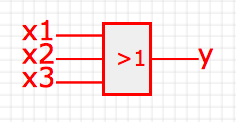
\includegraphics[width=7cm]{two_or_more.png}
\begin{center}
\begin{tabular}{ c | c | c | c }
  $x_1$ & $x_2$ & $x_3$ & $y$ \\ \hline
  0 & 0 & 0 & 0 \\
  0 & 0 & 1 & 0 \\
  0 & 1 & 0 & 0 \\
  0 & 1 & 1 & 1 \\
  1 & 0 & 0 & 0 \\
  1 & 0 & 1 & 1 \\
  1 & 1 & 0 & 1\\
  1 & 1 & 1 & 1 \\
\end{tabular}
\end{center}
Наиболее распространены элементы, выполняющие базовые логические операции. Кружочком у выхода обозначается инверсия.\\

%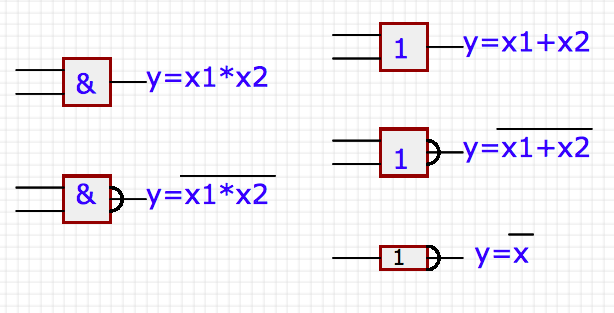
\includegraphics[width=12cm]{logical_operations.png}%

\begin{center}
\begin{circuitikz}
\draw (0,2.5) node [european and port] {И};
\draw (0,.5) node [european nand port] {И НЕ};
\draw (3, 3) node [european or port] {ИЛИ};
\draw (3, 1.5) node [european nor port] {ИЛИ НЕ};
\draw (3, 0) node [european not port] {НЕ};
\end{circuitikz}
\end{center}

Схемотехническая реализация:\\
Инвертор: \\
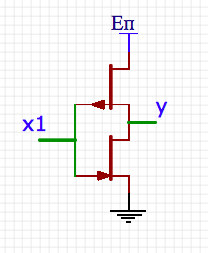
\includegraphics[width=5cm]{not.png}
И-НЕ:\\
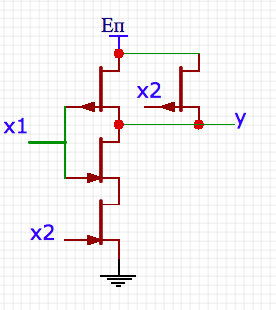
\includegraphics[width=7cm]{and_not.png}\\

\begin{center}
\begin{circuitikz}
\draw (0,0) node [ground] {}
node[njfet, anchor=S] (first) {}
(first.D) node[pjfet, anchor=D] (second) {}
(first.B)--(second.B)
(second.S) node[tground] {}
(second.S) node[above] {$E_\text{пит}$}
(first.D) to[short, -] ++(0.5, 0)
(first.D) node[above right] {$y$}
;\end{circuitikz}
\end{center}
\section{Способы задания логических функций}
\begin{enumerate}
\item Словесное описание:

если $x_1=x_2$, то $y=0$, $x_1 \not= x_2 \to y=1$
\item Таблица истинности:
\begin{tabular}{ c | c | c }
  $x_1$ & $x_2$ & $y$ \\ \hline
  0 & 0 & 0 \\
  0 & 1 & 1 \\
  1 & 0 & 1 \\
  1 & 1 & 0 \\
\end{tabular}
\item Структурная формула. Способы записи:

а) Совершенная дизъюнктивная нормальная формула

$y=f(x_1, x_2, x_3) \quad$
\begin{tabular}{ c | c | c | c }
  $x_1$ & $x_2$ & $x_3$ & $y$ \\ \hline
  0 & 0 & 0 & 0 \\
  0 & 0 & 1 & 0 \\
  0 & 1 & 0 & 0 \\
  0 & 1 & 1 & 1 \\
  1 & 0 & 0 & 0 \\
  1 & 0 & 1 & 1 \\
  1 & 1 & 0 & 1\\
  1 & 1 & 1 & 1 \\
\end{tabular}

Вводятся нормирующие функции $y_a, y_b, y_c, y_d$ (по количеству истинных значений $y$ таблице). Их значение - значение логического \textbf{И} от переменных, равных 1 или инвертированных: $y_a=\overline{x}_1x_2x_3, y_b=x_1\overline{x}_2x_3, y_c=x_1x_2\overline{x}_3, y_d=x_1x_2x_3$. Тогда $y=y_a+y_b+y_c+y_d$.

б) Совершенная конъюнктивная нормальная формула

Для той же функции $y$ можно ввести $y_e, y_f, y_g, y_h$. Берутся строки, где $y=0$, для них производится логическая сумма входных переменных, равных 0 или инвертированных. $y_e=x_1+x_2+x_3, y_f=\overline{x_1}+x_2+x_3, y_g=x_1+\overline{x_2}+x_3, y_h=x_1+x_2+\overline{x_3}$. Тогда $y=y_ey_fy_gy_h$.
\item Числовой способ задания функции

Для представления функции в СДНФ под знаком $\sum$ перечисляются номера наборов входных переменных, в которых функция равна 1.

$y(x_1, x_2, x_3)=\sum(3, 5, 6, 7)=\sum(011, 101, 110, 111)$\\

Для представления функции в СКНФ под знаком $\prod$ перечисляются номера наборов входных переменных, в которых функция равна 0.

$y(x_1, x_2, x_3)=\prod(0, 1, 2, 4)$
\end{enumerate}

\section{Переход от структурной формулы к логической схеме и обратно}
Элементы располагаются на схеме, начиная от входом, в том же порядке, в котором выполняются логические операции.

(сложная картинка с шиной)

Чтение СФ производится от выхода к входам: $y=\alpha+\beta+\gamma+\delta, \alpha=\overline{x_1}x_2x_3$. Поскольку для инвертора требуется 2 транзистора, для И - 8 транзисторов, а для ИЛИ - 10, всего для данной функции в КМОП технологии потребуется 48 транзисторов.

\section{Минимизация логических функций}
Построение логической схемы непосредственно по СФ (будь то СДНФ или СКНФ) нецелесообразно. Необходимо предварительно упростить формулу.
\begin{enumerate}
\item Метод Квайна (Quine) - операции склеивания ($x_1x_2+x_1\overline{x}_2=x_1$) и поглощения ($x_1x_2+x_1=x_1$). Предполагает 2 этапа: склеивание соседних слагаемых и поглощение избыточных слагаемых.

\textbf{Соседние слагаемые} - слагаемые, отличающиеся логическими значениями только одной переменной.

\begin{tabular}{ c | c | c | c | c | c}
  $x_1$ & $x_2$ & $x_3$ & $y_1$ & $y_2$ & $y_3$ \\ \hline
  0 & 0 & 0 & 1 & 1 & 0\\
  0 & 0 & 1 & 1 & 1 & 1\\
  0 & 1 & 0 & 0 & 1 & 0\\
  0 & 1 & 1 & 0 & 0 & 0\\
  1 & 0 & 0 & 0 & 0 & 0\\
  1 & 0 & 1 & 0 & 0 & 1\\
  1 & 1 & 0 & 0 & 0 & 1\\
  1 & 1 & 1 & 0 & 0 & 1\\
\end{tabular}
\begin{equation}
\left\{
\begin{aligned}
& y_1=\overline{x}_1\overline{x}_2\overline{x}_3+\overline{x}_3\overline{x}_2x_1=\overline{x}_2\overline{x}_3(\overline{x}_1+x_1)=\overline{x}_2\overline{x}_3 \\
& y_2= \overline{x}_1\overline{x}_2\overline{x}_3+\overline{x}_2\overline{x}_3x_1+x_1x_2x_3=\overline{x}_2\overline{x}_3+\overline{x}_1\overline{x}_3+x_1x_2x_3 \\
& y_3= \overline{x}_2\overline{x}_3x_1+ x_1\overline{x}_2+x_3+\overline{x}_1x_2x_3+x_1x_2x_3=\overline{x}_2x_1+x_3x_1+x_3x_2 = \overline{x}_2x_1+x_3x_2  \notag
\end{aligned}
\right.
\end{equation}

Недостатки метода - появление лишних слагаемых и экспоненциальный рост числа проверок склеивания при увеличеснии числа входных переменных.

$y_{mg}=\overline{x}_3x_2x_1+x_3\overline{x}_2x_1+x_3x_2\overline{x}_1+x_3x_2x_1=x_1x_2+x_2x_3+x_3x_1$ - (26 транзисторов в КМОП)

\item Метод Карно (Karnaugh)

Обеспечивает отсутствие лишних слагаемых благодаря наглядному представлению функции в виде карты.

Пример:
\begin{tabular}{ c | c | c }
  $x_1$ & $x_2$ & $y$ \\ \hline
  0 & 0 & 0 \\
  0 & 1 & 1 \\
  1 & 0 & 1 \\
  1 & 1 & 1 \\
\end{tabular}
\end{enumerate}
(далее на картинке)

Принципы: если в карте есть $2^N$ соседствующие (по горизонтали или вертикали) единицы, то они объединяются в группы. Цель: объединить все единицы минимальным количеством максимальных контуров.

Пример (из метода Квайна):
(картинка)
\begin{equation}
\left\{
\begin{aligned}
&y_1=\overline{x}_3\overline{x}_2\\
&y_2=\overline{x}_3\overline{x}_2+\overline{x}_3\overline{x}_1+x_1x_2x_3\\
&y_3=\overline{x}_2x_1+x_2x_3=(x_1+x_2)(x_3+\overline{x}_2)
\end{aligned}
\right.
\end{equation}

Пример: 3 контура
\begin{equation}
\left\{
\begin{aligned}
&y_1=\overline{x}_3\overline{x}_1\\
&y_2=\overline{x}_4x_3\\
&y_3=x_1x_2x_3=
\end{aligned}
\right.
\end{equation}

Пример: метод теряет наглядность.
\begin{tabular}{ c | c | c | c | c | c}
        & 00 & 01 & 10 & 11\\ \hline
  000 & 0 & 0 & 1 & 0 \\
  001 & 0 & 1 & 0 & 0\\
  011 & 1 & $\textbf{1}$ & 0 & 0\\
  010 & 1 & 0 & 0 & 0 \\  
  110 & 1 & 0 & 0 & 0 \\
  111 & 1 & $\textbf{1}$ & 0 & 0 \\
  101 & 0 & 1 & 0 & 0 \\
  100 & 0 & 0 & 0 & 0 \\
\end{tabular}
 Существует модифицированный метод Квайна-Маккласки, его сложность также эксп. возрастает,.
\end{document}

